% Options for packages loaded elsewhere
\PassOptionsToPackage{unicode}{hyperref}
\PassOptionsToPackage{hyphens}{url}
%
\documentclass[
]{article}
\usepackage{amsmath,amssymb}
\usepackage{lmodern}
\usepackage{iftex}
\ifPDFTeX
  \usepackage[T1]{fontenc}
  \usepackage[utf8]{inputenc}
  \usepackage{textcomp} % provide euro and other symbols
\else % if luatex or xetex
  \usepackage{unicode-math}
  \defaultfontfeatures{Scale=MatchLowercase}
  \defaultfontfeatures[\rmfamily]{Ligatures=TeX,Scale=1}
\fi
% Use upquote if available, for straight quotes in verbatim environments
\IfFileExists{upquote.sty}{\usepackage{upquote}}{}
\IfFileExists{microtype.sty}{% use microtype if available
  \usepackage[]{microtype}
  \UseMicrotypeSet[protrusion]{basicmath} % disable protrusion for tt fonts
}{}
\makeatletter
\@ifundefined{KOMAClassName}{% if non-KOMA class
  \IfFileExists{parskip.sty}{%
    \usepackage{parskip}
  }{% else
    \setlength{\parindent}{0pt}
    \setlength{\parskip}{6pt plus 2pt minus 1pt}}
}{% if KOMA class
  \KOMAoptions{parskip=half}}
\makeatother
\usepackage{xcolor}
\usepackage[margin=1in]{geometry}
\usepackage{color}
\usepackage{fancyvrb}
\newcommand{\VerbBar}{|}
\newcommand{\VERB}{\Verb[commandchars=\\\{\}]}
\DefineVerbatimEnvironment{Highlighting}{Verbatim}{commandchars=\\\{\}}
% Add ',fontsize=\small' for more characters per line
\usepackage{framed}
\definecolor{shadecolor}{RGB}{248,248,248}
\newenvironment{Shaded}{\begin{snugshade}}{\end{snugshade}}
\newcommand{\AlertTok}[1]{\textcolor[rgb]{0.94,0.16,0.16}{#1}}
\newcommand{\AnnotationTok}[1]{\textcolor[rgb]{0.56,0.35,0.01}{\textbf{\textit{#1}}}}
\newcommand{\AttributeTok}[1]{\textcolor[rgb]{0.77,0.63,0.00}{#1}}
\newcommand{\BaseNTok}[1]{\textcolor[rgb]{0.00,0.00,0.81}{#1}}
\newcommand{\BuiltInTok}[1]{#1}
\newcommand{\CharTok}[1]{\textcolor[rgb]{0.31,0.60,0.02}{#1}}
\newcommand{\CommentTok}[1]{\textcolor[rgb]{0.56,0.35,0.01}{\textit{#1}}}
\newcommand{\CommentVarTok}[1]{\textcolor[rgb]{0.56,0.35,0.01}{\textbf{\textit{#1}}}}
\newcommand{\ConstantTok}[1]{\textcolor[rgb]{0.00,0.00,0.00}{#1}}
\newcommand{\ControlFlowTok}[1]{\textcolor[rgb]{0.13,0.29,0.53}{\textbf{#1}}}
\newcommand{\DataTypeTok}[1]{\textcolor[rgb]{0.13,0.29,0.53}{#1}}
\newcommand{\DecValTok}[1]{\textcolor[rgb]{0.00,0.00,0.81}{#1}}
\newcommand{\DocumentationTok}[1]{\textcolor[rgb]{0.56,0.35,0.01}{\textbf{\textit{#1}}}}
\newcommand{\ErrorTok}[1]{\textcolor[rgb]{0.64,0.00,0.00}{\textbf{#1}}}
\newcommand{\ExtensionTok}[1]{#1}
\newcommand{\FloatTok}[1]{\textcolor[rgb]{0.00,0.00,0.81}{#1}}
\newcommand{\FunctionTok}[1]{\textcolor[rgb]{0.00,0.00,0.00}{#1}}
\newcommand{\ImportTok}[1]{#1}
\newcommand{\InformationTok}[1]{\textcolor[rgb]{0.56,0.35,0.01}{\textbf{\textit{#1}}}}
\newcommand{\KeywordTok}[1]{\textcolor[rgb]{0.13,0.29,0.53}{\textbf{#1}}}
\newcommand{\NormalTok}[1]{#1}
\newcommand{\OperatorTok}[1]{\textcolor[rgb]{0.81,0.36,0.00}{\textbf{#1}}}
\newcommand{\OtherTok}[1]{\textcolor[rgb]{0.56,0.35,0.01}{#1}}
\newcommand{\PreprocessorTok}[1]{\textcolor[rgb]{0.56,0.35,0.01}{\textit{#1}}}
\newcommand{\RegionMarkerTok}[1]{#1}
\newcommand{\SpecialCharTok}[1]{\textcolor[rgb]{0.00,0.00,0.00}{#1}}
\newcommand{\SpecialStringTok}[1]{\textcolor[rgb]{0.31,0.60,0.02}{#1}}
\newcommand{\StringTok}[1]{\textcolor[rgb]{0.31,0.60,0.02}{#1}}
\newcommand{\VariableTok}[1]{\textcolor[rgb]{0.00,0.00,0.00}{#1}}
\newcommand{\VerbatimStringTok}[1]{\textcolor[rgb]{0.31,0.60,0.02}{#1}}
\newcommand{\WarningTok}[1]{\textcolor[rgb]{0.56,0.35,0.01}{\textbf{\textit{#1}}}}
\usepackage{longtable,booktabs,array}
\usepackage{calc} % for calculating minipage widths
% Correct order of tables after \paragraph or \subparagraph
\usepackage{etoolbox}
\makeatletter
\patchcmd\longtable{\par}{\if@noskipsec\mbox{}\fi\par}{}{}
\makeatother
% Allow footnotes in longtable head/foot
\IfFileExists{footnotehyper.sty}{\usepackage{footnotehyper}}{\usepackage{footnote}}
\makesavenoteenv{longtable}
\usepackage{graphicx}
\makeatletter
\def\maxwidth{\ifdim\Gin@nat@width>\linewidth\linewidth\else\Gin@nat@width\fi}
\def\maxheight{\ifdim\Gin@nat@height>\textheight\textheight\else\Gin@nat@height\fi}
\makeatother
% Scale images if necessary, so that they will not overflow the page
% margins by default, and it is still possible to overwrite the defaults
% using explicit options in \includegraphics[width, height, ...]{}
\setkeys{Gin}{width=\maxwidth,height=\maxheight,keepaspectratio}
% Set default figure placement to htbp
\makeatletter
\def\fps@figure{htbp}
\makeatother
\setlength{\emergencystretch}{3em} % prevent overfull lines
\providecommand{\tightlist}{%
  \setlength{\itemsep}{0pt}\setlength{\parskip}{0pt}}
\setcounter{secnumdepth}{-\maxdimen} % remove section numbering
\usepackage{amsmath}
\usepackage{booktabs}
\usepackage{caption}
\usepackage{longtable}
\ifLuaTeX
  \usepackage{selnolig}  % disable illegal ligatures
\fi
\IfFileExists{bookmark.sty}{\usepackage{bookmark}}{\usepackage{hyperref}}
\IfFileExists{xurl.sty}{\usepackage{xurl}}{} % add URL line breaks if available
\urlstyle{same} % disable monospaced font for URLs
\hypersetup{
  pdftitle={Lab 5 - part 1},
  pdfauthor={Erica Bishop (and Jillian Allison)},
  hidelinks,
  pdfcreator={LaTeX via pandoc}}

\title{Lab 5 - part 1}
\author{Erica Bishop (and Jillian Allison)}
\date{2023-02-07}

\begin{document}
\maketitle

This week's lab is a musical lab. You'll be requesting data from the
Spotify API and using it to build k-nearest neighbor and decision tree
models.

In order to use the Spotify you must have a Spotify account. If you
don't have one, sign up for a free one here:
\url{https://www.spotify.com/us/signup}

Once you have an account, go to Spotify for developers
(\url{https://developer.spotify.com/}) and log in. Click the green
``Create a Client ID'' button to fill out the form to create an app
create an app so you can access the API.

On your developer dashboard page, click on the new app you just created.
On the app's dashboard page you will find your Client ID just under the
header name of your app. Click ``Show Client Secret'' to access your
secondary Client ID. When you do this you'll be issued a Spotify client
ID and client secret key.

You have two options for completing this lab.

\textbf{Option 1}: \textbf{Classify by users}. Build models that predict
whether a given song will be in your collection vs.~a partner in class.
This requires that you were already a Spotify user so you have enough
data to work with. You will download your data from the Spotify API and
then exchange with another member of class.

\textbf{Option 2}: \textbf{Classify by genres}. Build models that
predict which genre a song belongs to. This will use a pre-existing
Spotify dataset available from Kaggle.com
(\url{https://www.kaggle.com/datasets/mrmorj/dataset-of-songs-in-spotify})

\begin{Shaded}
\begin{Highlighting}[]
\FunctionTok{library}\NormalTok{(spotifyr) }\CommentTok{\#API interaction}
\FunctionTok{library}\NormalTok{(tidyverse)}
\end{Highlighting}
\end{Shaded}

\begin{verbatim}
## -- Attaching packages --------------------------------------- tidyverse 1.3.2 --
## v ggplot2 3.3.6     v purrr   0.3.4
## v tibble  3.1.8     v dplyr   1.0.9
## v tidyr   1.2.0     v stringr 1.4.1
## v readr   2.1.2     v forcats 0.5.1
## -- Conflicts ------------------------------------------ tidyverse_conflicts() --
## x dplyr::filter() masks stats::filter()
## x dplyr::lag()    masks stats::lag()
\end{verbatim}

\begin{Shaded}
\begin{Highlighting}[]
\FunctionTok{library}\NormalTok{(tidymodels)}
\end{Highlighting}
\end{Shaded}

\begin{verbatim}
## -- Attaching packages -------------------------------------- tidymodels 1.0.0 --
## v broom        1.0.0     v rsample      1.1.0
## v dials        1.0.0     v tune         1.0.0
## v infer        1.0.3     v workflows    1.0.0
## v modeldata    1.0.1     v workflowsets 1.0.0
## v parsnip      1.0.1     v yardstick    1.1.0
## v recipes      1.0.1     
## -- Conflicts ----------------------------------------- tidymodels_conflicts() --
## x scales::discard() masks purrr::discard()
## x dplyr::filter()   masks stats::filter()
## x recipes::fixed()  masks stringr::fixed()
## x dplyr::lag()      masks stats::lag()
## x yardstick::spec() masks readr::spec()
## x recipes::step()   masks stats::step()
## * Use tidymodels_prefer() to resolve common conflicts.
\end{verbatim}

\begin{Shaded}
\begin{Highlighting}[]
\FunctionTok{library}\NormalTok{(gt)}
\FunctionTok{library}\NormalTok{(here)}
\end{Highlighting}
\end{Shaded}

\begin{verbatim}
## here() starts at /Users/ericabishop/Documents/MEDSwinter/EDS232-ml/eds232labs
\end{verbatim}

\begin{Shaded}
\begin{Highlighting}[]
\FunctionTok{library}\NormalTok{(patchwork)}
\FunctionTok{library}\NormalTok{(tune)}
\FunctionTok{library}\NormalTok{(baguette)}
\FunctionTok{library}\NormalTok{(doParallel)}
\end{Highlighting}
\end{Shaded}

\begin{verbatim}
## Loading required package: foreach
## 
## Attaching package: 'foreach'
## 
## The following objects are masked from 'package:purrr':
## 
##     accumulate, when
## 
## Loading required package: iterators
## Loading required package: parallel
\end{verbatim}

\begin{Shaded}
\begin{Highlighting}[]
\FunctionTok{library}\NormalTok{(ranger)}
\end{Highlighting}
\end{Shaded}

Client ID and Client Secret are required to create and access token that
is required to interact with the API. You can set them as system values
so we don't have to do provide them each time.

Sys.setenv(SPOTIFY\_CLIENT\_ID = `2e066a0ebf86473990f30eee626c4ab9')
Sys.setenv(SPOTIFY\_CLIENT\_SECRET = `bb6735cb728a42089e0cc02680c97844')

access\_token \textless- get\_spotify\_access\_token() \#takes ID and
SECRET, sends to Spotify and receives an access token

\begin{quote}
\emph{This may result in an error:}

INVALID\_CLIENT: Invalid redirect URI

\emph{This can be resolved by editing the callback settings on your app.
Go to your app and click ``Edit Settings''. Under redirect URLs paste
this: \url{http://localhost:1410/} and click save at the bottom.}
\end{quote}

\textbf{Option 1: Data Preparation}

You can use get\_my\_saved\_tracks() to request all your liked tracks.
It would be good if you had at least 150-200 liked tracks so the model
has enough data to work with. If you don't have enough liked tracks, you
can instead use get\_my\_recently\_played(), and in that case grab at
least 500 recently played tracks if you can.

The Spotify API returns a dataframe of tracks and associated attributes.
However, it will only return up to 50 (or 20) tracks at a time, so you
will have to make multiple requests. Use a function to combine all your
requests in one call.

Once you have your tracks, familiarize yourself with this initial
dataframe. You'll need to request some additional information for the
analysis. If you give the API a list of track IDs using
get\_track\_audio\_features(), it will return an audio features
dataframe of all the tracks and some attributes of them.

These track audio features are the predictors we are interested in, but
this dataframe doesn't have the actual names of the tracks. Append the
`track.name' column from your favorite tracks database.

Find a class mate whose data you would like to use. Add your partner's
data to your dataset. Create a new column that will contain the outcome
variable that you will try to predict. This variable should contain two
values that represent if the track came from your data set or your
partner's.

\textbf{Option 2: Data preparation}

Download the Spotify dataset from
\url{https://www.kaggle.com/datasets/mrmorj/dataset-of-songs-in-spotify}

Inspect the data. Choose two genres you'd like to use for the
classification task. Filter down the data to include only the tracks of
that genre.

\textbf{see the r script lab5\_get\_spotify\_data.R for accessing data
via spotify API.} Below I read in the data I pulled from spotify, and
saved the API calls and data manipulation in a separate script to make
knitting faster for this markdown file.

\begin{Shaded}
\begin{Highlighting}[]
\CommentTok{\#read in data (saved as csv from r script code)}
\NormalTok{eb\_tracks\_df }\OtherTok{\textless{}{-}} \FunctionTok{read\_csv}\NormalTok{(}\FunctionTok{here}\NormalTok{(}\StringTok{"eb\_track\_attributes.csv"}\NormalTok{))}
\end{Highlighting}
\end{Shaded}

\begin{verbatim}
## Rows: 2950 Columns: 20
## -- Column specification --------------------------------------------------------
## Delimiter: ","
## chr  (7): type, id, uri, track_href, analysis_url, track.name, user
## dbl (13): danceability, energy, key, loudness, mode, speechiness, acousticne...
## 
## i Use `spec()` to retrieve the full column specification for this data.
## i Specify the column types or set `show_col_types = FALSE` to quiet this message.
\end{verbatim}

\begin{Shaded}
\begin{Highlighting}[]
\CommentTok{\#read in Jillian\textquotesingle{}s data}
\NormalTok{ja\_tracks\_df }\OtherTok{\textless{}{-}} \FunctionTok{read\_csv}\NormalTok{(}\FunctionTok{here}\NormalTok{(}\StringTok{"jillian\_spotify\_data.csv"}\NormalTok{)) }\SpecialCharTok{|\textgreater{}} 
  \FunctionTok{select}\NormalTok{(}\SpecialCharTok{{-}}\NormalTok{track\_id) }\SpecialCharTok{|\textgreater{}} \CommentTok{\#drop track\_id column (repeats id column)}
  \FunctionTok{rename}\NormalTok{(}\AttributeTok{track.name =}\NormalTok{ track\_name)}\CommentTok{\#renametrack\_name to match}
\end{Highlighting}
\end{Shaded}

\begin{verbatim}
## Rows: 931 Columns: 21
## -- Column specification --------------------------------------------------------
## Delimiter: ","
## chr  (8): type, id, uri, track_href, analysis_url, track_name, track_id, user
## dbl (13): danceability, energy, key, loudness, mode, speechiness, acousticne...
## 
## i Use `spec()` to retrieve the full column specification for this data.
## i Specify the column types or set `show_col_types = FALSE` to quiet this message.
\end{verbatim}

\#\#Data Exploration (both options)

Let's take a look at your data. Do some exploratory summary stats and
visualization.

For example: What are the most danceable tracks in your dataset? What
are some differences in the data between users (Option 1) or genres
(Option 2)?

\begin{Shaded}
\begin{Highlighting}[]
\CommentTok{\#skim both datasets}
\NormalTok{skimr}\SpecialCharTok{::}\FunctionTok{skim}\NormalTok{(eb\_tracks\_df)}
\end{Highlighting}
\end{Shaded}

\begin{longtable}[]{@{}ll@{}}
\caption{Data summary}\tabularnewline
\toprule()
\endhead
Name & eb\_tracks\_df \\
Number of rows & 2950 \\
Number of columns & 20 \\
\_\_\_\_\_\_\_\_\_\_\_\_\_\_\_\_\_\_\_\_\_\_\_ & \\
Column type frequency: & \\
character & 7 \\
numeric & 13 \\
\_\_\_\_\_\_\_\_\_\_\_\_\_\_\_\_\_\_\_\_\_\_\_\_ & \\
Group variables & None \\
\bottomrule()
\end{longtable}

\textbf{Variable type: character}

\begin{longtable}[]{@{}
  >{\raggedright\arraybackslash}p{(\columnwidth - 14\tabcolsep) * \real{0.1944}}
  >{\raggedleft\arraybackslash}p{(\columnwidth - 14\tabcolsep) * \real{0.1389}}
  >{\raggedleft\arraybackslash}p{(\columnwidth - 14\tabcolsep) * \real{0.1944}}
  >{\raggedleft\arraybackslash}p{(\columnwidth - 14\tabcolsep) * \real{0.0556}}
  >{\raggedleft\arraybackslash}p{(\columnwidth - 14\tabcolsep) * \real{0.0556}}
  >{\raggedleft\arraybackslash}p{(\columnwidth - 14\tabcolsep) * \real{0.0833}}
  >{\raggedleft\arraybackslash}p{(\columnwidth - 14\tabcolsep) * \real{0.1250}}
  >{\raggedleft\arraybackslash}p{(\columnwidth - 14\tabcolsep) * \real{0.1528}}@{}}
\toprule()
\begin{minipage}[b]{\linewidth}\raggedright
skim\_variable
\end{minipage} & \begin{minipage}[b]{\linewidth}\raggedleft
n\_missing
\end{minipage} & \begin{minipage}[b]{\linewidth}\raggedleft
complete\_rate
\end{minipage} & \begin{minipage}[b]{\linewidth}\raggedleft
min
\end{minipage} & \begin{minipage}[b]{\linewidth}\raggedleft
max
\end{minipage} & \begin{minipage}[b]{\linewidth}\raggedleft
empty
\end{minipage} & \begin{minipage}[b]{\linewidth}\raggedleft
n\_unique
\end{minipage} & \begin{minipage}[b]{\linewidth}\raggedleft
whitespace
\end{minipage} \\
\midrule()
\endhead
type & 0 & 1 & 14 & 14 & 0 & 1 & 0 \\
id & 0 & 1 & 22 & 22 & 0 & 2950 & 0 \\
uri & 0 & 1 & 36 & 36 & 0 & 2950 & 0 \\
track\_href & 0 & 1 & 56 & 56 & 0 & 2950 & 0 \\
analysis\_url & 0 & 1 & 64 & 64 & 0 & 2950 & 0 \\
track.name & 0 & 1 & 1 & 139 & 0 & 2780 & 0 \\
user & 0 & 1 & 5 & 5 & 0 & 1 & 0 \\
\bottomrule()
\end{longtable}

\textbf{Variable type: numeric}

\begin{longtable}[]{@{}
  >{\raggedright\arraybackslash}p{(\columnwidth - 20\tabcolsep) * \real{0.1466}}
  >{\raggedleft\arraybackslash}p{(\columnwidth - 20\tabcolsep) * \real{0.0862}}
  >{\raggedleft\arraybackslash}p{(\columnwidth - 20\tabcolsep) * \real{0.1207}}
  >{\raggedleft\arraybackslash}p{(\columnwidth - 20\tabcolsep) * \real{0.0862}}
  >{\raggedleft\arraybackslash}p{(\columnwidth - 20\tabcolsep) * \real{0.0776}}
  >{\raggedleft\arraybackslash}p{(\columnwidth - 20\tabcolsep) * \real{0.0776}}
  >{\raggedleft\arraybackslash}p{(\columnwidth - 20\tabcolsep) * \real{0.0862}}
  >{\raggedleft\arraybackslash}p{(\columnwidth - 20\tabcolsep) * \real{0.0862}}
  >{\raggedleft\arraybackslash}p{(\columnwidth - 20\tabcolsep) * \real{0.0862}}
  >{\raggedleft\arraybackslash}p{(\columnwidth - 20\tabcolsep) * \real{0.0948}}
  >{\raggedright\arraybackslash}p{(\columnwidth - 20\tabcolsep) * \real{0.0517}}@{}}
\toprule()
\begin{minipage}[b]{\linewidth}\raggedright
skim\_variable
\end{minipage} & \begin{minipage}[b]{\linewidth}\raggedleft
n\_missing
\end{minipage} & \begin{minipage}[b]{\linewidth}\raggedleft
complete\_rate
\end{minipage} & \begin{minipage}[b]{\linewidth}\raggedleft
mean
\end{minipage} & \begin{minipage}[b]{\linewidth}\raggedleft
sd
\end{minipage} & \begin{minipage}[b]{\linewidth}\raggedleft
p0
\end{minipage} & \begin{minipage}[b]{\linewidth}\raggedleft
p25
\end{minipage} & \begin{minipage}[b]{\linewidth}\raggedleft
p50
\end{minipage} & \begin{minipage}[b]{\linewidth}\raggedleft
p75
\end{minipage} & \begin{minipage}[b]{\linewidth}\raggedleft
p100
\end{minipage} & \begin{minipage}[b]{\linewidth}\raggedright
hist
\end{minipage} \\
\midrule()
\endhead
danceability & 0 & 1 & 0.60 & 0.15 & 0.07 & 0.50 & 0.61 & 0.71 & 0.97 &
▁▂▇▇▂ \\
energy & 0 & 1 & 0.54 & 0.20 & 0.00 & 0.41 & 0.55 & 0.69 & 0.98 &
▂▃▇▇▂ \\
key & 0 & 1 & 5.19 & 3.55 & 0.00 & 2.00 & 5.00 & 8.00 & 11.00 & ▇▃▅▅▆ \\
loudness & 0 & 1 & -8.72 & 4.03 & -39.33 & -10.33 & -7.88 & -6.13 &
-1.28 & ▁▁▁▅▇ \\
mode & 0 & 1 & 0.68 & 0.47 & 0.00 & 0.00 & 1.00 & 1.00 & 1.00 & ▃▁▁▁▇ \\
speechiness & 0 & 1 & 0.09 & 0.11 & 0.02 & 0.03 & 0.05 & 0.10 & 0.95 &
▇▁▁▁▁ \\
acousticness & 0 & 1 & 0.37 & 0.31 & 0.00 & 0.08 & 0.29 & 0.64 & 1.00 &
▇▃▃▃▂ \\
instrumentalness & 0 & 1 & 0.07 & 0.20 & 0.00 & 0.00 & 0.00 & 0.01 &
0.98 & ▇▁▁▁▁ \\
liveness & 0 & 1 & 0.18 & 0.14 & 0.02 & 0.10 & 0.12 & 0.21 & 0.96 &
▇▂▁▁▁ \\
valence & 0 & 1 & 0.44 & 0.23 & 0.03 & 0.26 & 0.42 & 0.60 & 0.98 &
▅▇▇▅▂ \\
tempo & 0 & 1 & 116.77 & 28.92 & 45.31 & 93.97 & 115.21 & 134.93 &
241.05 & ▂▇▅▁▁ \\
duration\_ms & 0 & 1 & 222520.55 & 65886.74 & 25987.00 & 184762.00 &
214967.00 & 251068.50 & 1147000.00 & ▇▃▁▁▁ \\
time\_signature & 0 & 1 & 3.91 & 0.40 & 1.00 & 4.00 & 4.00 & 4.00 & 5.00
& ▁▁▁▇▁ \\
\bottomrule()
\end{longtable}

\begin{Shaded}
\begin{Highlighting}[]
\NormalTok{skimr}\SpecialCharTok{::}\FunctionTok{skim}\NormalTok{(ja\_tracks\_df)}
\end{Highlighting}
\end{Shaded}

\begin{longtable}[]{@{}ll@{}}
\caption{Data summary}\tabularnewline
\toprule()
\endhead
Name & ja\_tracks\_df \\
Number of rows & 931 \\
Number of columns & 20 \\
\_\_\_\_\_\_\_\_\_\_\_\_\_\_\_\_\_\_\_\_\_\_\_ & \\
Column type frequency: & \\
character & 7 \\
numeric & 13 \\
\_\_\_\_\_\_\_\_\_\_\_\_\_\_\_\_\_\_\_\_\_\_\_\_ & \\
Group variables & None \\
\bottomrule()
\end{longtable}

\textbf{Variable type: character}

\begin{longtable}[]{@{}
  >{\raggedright\arraybackslash}p{(\columnwidth - 14\tabcolsep) * \real{0.1944}}
  >{\raggedleft\arraybackslash}p{(\columnwidth - 14\tabcolsep) * \real{0.1389}}
  >{\raggedleft\arraybackslash}p{(\columnwidth - 14\tabcolsep) * \real{0.1944}}
  >{\raggedleft\arraybackslash}p{(\columnwidth - 14\tabcolsep) * \real{0.0556}}
  >{\raggedleft\arraybackslash}p{(\columnwidth - 14\tabcolsep) * \real{0.0556}}
  >{\raggedleft\arraybackslash}p{(\columnwidth - 14\tabcolsep) * \real{0.0833}}
  >{\raggedleft\arraybackslash}p{(\columnwidth - 14\tabcolsep) * \real{0.1250}}
  >{\raggedleft\arraybackslash}p{(\columnwidth - 14\tabcolsep) * \real{0.1528}}@{}}
\toprule()
\begin{minipage}[b]{\linewidth}\raggedright
skim\_variable
\end{minipage} & \begin{minipage}[b]{\linewidth}\raggedleft
n\_missing
\end{minipage} & \begin{minipage}[b]{\linewidth}\raggedleft
complete\_rate
\end{minipage} & \begin{minipage}[b]{\linewidth}\raggedleft
min
\end{minipage} & \begin{minipage}[b]{\linewidth}\raggedleft
max
\end{minipage} & \begin{minipage}[b]{\linewidth}\raggedleft
empty
\end{minipage} & \begin{minipage}[b]{\linewidth}\raggedleft
n\_unique
\end{minipage} & \begin{minipage}[b]{\linewidth}\raggedleft
whitespace
\end{minipage} \\
\midrule()
\endhead
type & 0 & 1 & 14 & 14 & 0 & 1 & 0 \\
id & 0 & 1 & 22 & 22 & 0 & 931 & 0 \\
uri & 0 & 1 & 36 & 36 & 0 & 931 & 0 \\
track\_href & 0 & 1 & 56 & 56 & 0 & 931 & 0 \\
analysis\_url & 0 & 1 & 64 & 64 & 0 & 931 & 0 \\
track.name & 0 & 1 & 2 & 68 & 0 & 881 & 0 \\
user & 0 & 1 & 7 & 7 & 0 & 1 & 0 \\
\bottomrule()
\end{longtable}

\textbf{Variable type: numeric}

\begin{longtable}[]{@{}
  >{\raggedright\arraybackslash}p{(\columnwidth - 20\tabcolsep) * \real{0.1532}}
  >{\raggedleft\arraybackslash}p{(\columnwidth - 20\tabcolsep) * \real{0.0901}}
  >{\raggedleft\arraybackslash}p{(\columnwidth - 20\tabcolsep) * \real{0.1261}}
  >{\raggedleft\arraybackslash}p{(\columnwidth - 20\tabcolsep) * \real{0.0901}}
  >{\raggedleft\arraybackslash}p{(\columnwidth - 20\tabcolsep) * \real{0.0811}}
  >{\raggedleft\arraybackslash}p{(\columnwidth - 20\tabcolsep) * \real{0.0450}}
  >{\raggedleft\arraybackslash}p{(\columnwidth - 20\tabcolsep) * \real{0.0901}}
  >{\raggedleft\arraybackslash}p{(\columnwidth - 20\tabcolsep) * \real{0.0901}}
  >{\raggedleft\arraybackslash}p{(\columnwidth - 20\tabcolsep) * \real{0.0901}}
  >{\raggedleft\arraybackslash}p{(\columnwidth - 20\tabcolsep) * \real{0.0901}}
  >{\raggedright\arraybackslash}p{(\columnwidth - 20\tabcolsep) * \real{0.0541}}@{}}
\toprule()
\begin{minipage}[b]{\linewidth}\raggedright
skim\_variable
\end{minipage} & \begin{minipage}[b]{\linewidth}\raggedleft
n\_missing
\end{minipage} & \begin{minipage}[b]{\linewidth}\raggedleft
complete\_rate
\end{minipage} & \begin{minipage}[b]{\linewidth}\raggedleft
mean
\end{minipage} & \begin{minipage}[b]{\linewidth}\raggedleft
sd
\end{minipage} & \begin{minipage}[b]{\linewidth}\raggedleft
p0
\end{minipage} & \begin{minipage}[b]{\linewidth}\raggedleft
p25
\end{minipage} & \begin{minipage}[b]{\linewidth}\raggedleft
p50
\end{minipage} & \begin{minipage}[b]{\linewidth}\raggedleft
p75
\end{minipage} & \begin{minipage}[b]{\linewidth}\raggedleft
p100
\end{minipage} & \begin{minipage}[b]{\linewidth}\raggedright
hist
\end{minipage} \\
\midrule()
\endhead
danceability & 0 & 1 & 0.58 & 0.16 & 0 & 0.47 & 0.59 & 0.70 & 0.95 &
▁▂▇▇▂ \\
energy & 0 & 1 & 0.59 & 0.21 & 0 & 0.44 & 0.60 & 0.76 & 0.96 & ▁▃▇▇▆ \\
key & 0 & 1 & 5.18 & 3.62 & 0 & 2.00 & 5.00 & 8.00 & 11.00 & ▇▂▃▅▆ \\
loudness & 0 & 1 & -8.46 & 3.85 & -60 & -10.37 & -7.81 & -5.93 & 1.13 &
▁▁▁▂▇ \\
mode & 0 & 1 & 0.58 & 0.49 & 0 & 0.00 & 1.00 & 1.00 & 1.00 & ▆▁▁▁▇ \\
speechiness & 0 & 1 & 0.17 & 0.25 & 0 & 0.04 & 0.06 & 0.16 & 0.96 &
▇▁▁▁▁ \\
acousticness & 0 & 1 & 0.37 & 0.33 & 0 & 0.06 & 0.27 & 0.71 & 1.00 &
▇▃▂▃▃ \\
instrumentalness & 0 & 1 & 0.05 & 0.18 & 0 & 0.00 & 0.00 & 0.00 & 0.94 &
▇▁▁▁▁ \\
liveness & 0 & 1 & 0.24 & 0.23 & 0 & 0.10 & 0.14 & 0.30 & 0.99 &
▇▂▁▁▁ \\
valence & 0 & 1 & 0.46 & 0.25 & 0 & 0.27 & 0.43 & 0.64 & 0.98 & ▅▇▇▅▃ \\
tempo & 0 & 1 & 115.09 & 30.42 & 0 & 92.58 & 113.12 & 133.92 & 211.42 &
▁▂▇▃▁ \\
duration\_ms & 0 & 1 & 215737.63 & 75300.76 & 4800 & 177227.00 &
214747.00 & 252103.50 & 592920.00 & ▁▇▃▁▁ \\
time\_signature & 0 & 1 & 3.87 & 0.52 & 0 & 4.00 & 4.00 & 4.00 & 5.00 &
▁▁▁▇▁ \\
\bottomrule()
\end{longtable}

\begin{Shaded}
\begin{Highlighting}[]
\CommentTok{\#take a closer look at some variables}
\FunctionTok{names}\NormalTok{(eb\_tracks\_df)}
\end{Highlighting}
\end{Shaded}

\begin{verbatim}
##  [1] "danceability"     "energy"           "key"              "loudness"        
##  [5] "mode"             "speechiness"      "acousticness"     "instrumentalness"
##  [9] "liveness"         "valence"          "tempo"            "type"            
## [13] "id"               "uri"              "track_href"       "analysis_url"    
## [17] "duration_ms"      "time_signature"   "track.name"       "user"
\end{verbatim}

\begin{Shaded}
\begin{Highlighting}[]
\FunctionTok{names}\NormalTok{(ja\_tracks\_df)}
\end{Highlighting}
\end{Shaded}

\begin{verbatim}
##  [1] "danceability"     "energy"           "key"              "loudness"        
##  [5] "mode"             "speechiness"      "acousticness"     "instrumentalness"
##  [9] "liveness"         "valence"          "tempo"            "type"            
## [13] "id"               "uri"              "track_href"       "analysis_url"    
## [17] "duration_ms"      "time_signature"   "track.name"       "user"
\end{verbatim}

\begin{Shaded}
\begin{Highlighting}[]
\CommentTok{\#do we have any of the same tracks saved??}
\NormalTok{eb\_ja\_shared\_faves }\OtherTok{\textless{}{-}} \FunctionTok{semi\_join}\NormalTok{(eb\_tracks\_df, ja\_tracks\_df, }\AttributeTok{by =} \StringTok{"id"}\NormalTok{) }\CommentTok{\#use semi\_join to get df of tracks in common}
\CommentTok{\#looks like a lot of beyonce, frank ocean, and lady gaga, but let\textquotesingle{}s take a closer look!}

\CommentTok{\#what are the characteristics of our shared tracks?}
\NormalTok{eb\_ja\_summary }\OtherTok{\textless{}{-}}\NormalTok{ eb\_ja\_shared\_faves }\SpecialCharTok{|\textgreater{}} 
  \FunctionTok{select}\NormalTok{(danceability, energy, key, valence, loudness, speechiness, acousticness) }\SpecialCharTok{|\textgreater{}} 
  \FunctionTok{summarise\_all}\NormalTok{(mean) }\SpecialCharTok{|\textgreater{}} \CommentTok{\#calculate the average of some variables of interest}
  \FunctionTok{add\_column}\NormalTok{(}\AttributeTok{user =} \StringTok{"both \textless{}3"}\NormalTok{) }\CommentTok{\#update user column to show both of us}

\CommentTok{\#compare the characteristics of shared tracks to just mine}
\NormalTok{eb\_summary }\OtherTok{\textless{}{-}}\NormalTok{ eb\_tracks\_df }\SpecialCharTok{|\textgreater{}} 
  \FunctionTok{select}\NormalTok{(danceability, energy, key, valence, loudness, speechiness, acousticness) }\SpecialCharTok{|\textgreater{}} 
  \FunctionTok{summarise\_all}\NormalTok{(mean) }\SpecialCharTok{|\textgreater{}} 
  \FunctionTok{add\_column}\NormalTok{(}\AttributeTok{user =} \StringTok{"Erica"}\NormalTok{)}

\CommentTok{\#calculate same summary table for jillian}
\NormalTok{ja\_summary }\OtherTok{\textless{}{-}}\NormalTok{ ja\_tracks\_df }\SpecialCharTok{|\textgreater{}} 
  \FunctionTok{select}\NormalTok{(danceability, energy, key, valence, loudness, speechiness, acousticness) }\SpecialCharTok{|\textgreater{}} 
  \FunctionTok{summarise\_all}\NormalTok{(mean) }\SpecialCharTok{|\textgreater{}} 
  \FunctionTok{add\_column}\NormalTok{(}\AttributeTok{user =} \StringTok{"Jillian"}\NormalTok{)}

\CommentTok{\#combine the summary stats tables into one df }
\NormalTok{summary\_df }\OtherTok{\textless{}{-}} \FunctionTok{rbind}\NormalTok{(eb\_ja\_summary, eb\_summary, ja\_summary)}

\FunctionTok{gt}\NormalTok{(summary\_df) }\CommentTok{\#print as table}
\end{Highlighting}
\end{Shaded}

\begin{longtable}{rrrrrrrl}
\toprule
danceability & energy & key & valence & loudness & speechiness & acousticness & user \\ 
\midrule
0.5447193 & 0.4883711 & 5.438596 & 0.4066061 & -8.986886 & 0.10642895 & 0.4252122 & both <3 \\ 
0.5995531 & 0.5372327 & 5.187458 & 0.4405259 & -8.716053 & 0.09319224 & 0.3696987 & Erica \\ 
0.5809903 & 0.5887244 & 5.178303 & 0.4569398 & -8.457608 & 0.17055134 & 0.3743012 & Jillian \\ 
\bottomrule
\end{longtable}

\begin{Shaded}
\begin{Highlighting}[]
\CommentTok{\#combine both data sets}

\NormalTok{eb\_ja\_tracks }\OtherTok{\textless{}{-}} \FunctionTok{full\_join}\NormalTok{(eb\_tracks\_df,}
\NormalTok{                          ja\_tracks\_df,}
                          \AttributeTok{by =} \FunctionTok{c}\NormalTok{(}\StringTok{"danceability"}\NormalTok{, }\StringTok{"energy"}\NormalTok{, }\StringTok{"key"}\NormalTok{, }\StringTok{"loudness"}\NormalTok{, }\StringTok{"mode"}\NormalTok{, }\StringTok{"speechiness"}\NormalTok{, }\StringTok{"acousticness"}\NormalTok{, }\StringTok{"instrumentalness"}\NormalTok{, }\StringTok{"liveness"}\NormalTok{, }\StringTok{"valence"}\NormalTok{, }\StringTok{"tempo"}\NormalTok{, }\StringTok{"type"}\NormalTok{, }\StringTok{"id"}\NormalTok{, }\StringTok{"uri"}\NormalTok{, }\StringTok{"track\_href"}\NormalTok{, }\StringTok{"analysis\_url"}\NormalTok{, }\StringTok{"duration\_ms"}\NormalTok{, }\StringTok{"time\_signature"}\NormalTok{, }\StringTok{"track.name"}\NormalTok{)) }\SpecialCharTok{|\textgreater{}} 
  \FunctionTok{mutate}\NormalTok{(}\AttributeTok{user =} \FunctionTok{case\_when}\NormalTok{(}
\NormalTok{    user.y }\SpecialCharTok{==} \StringTok{"Jillian"} \SpecialCharTok{\&}\NormalTok{ user.x }\SpecialCharTok{==} \StringTok{"Erica"} \SpecialCharTok{\textasciitilde{}} \StringTok{"Both"}\NormalTok{, }\CommentTok{\#relabel songs in both user lists with case\_when}
\NormalTok{    user.y }\SpecialCharTok{==} \StringTok{"Jillian"} \SpecialCharTok{\&} \FunctionTok{is.na}\NormalTok{(user.x) }\SpecialCharTok{\textasciitilde{}} \StringTok{"Jillian"}\NormalTok{,}
    \ConstantTok{TRUE} \SpecialCharTok{\textasciitilde{}} \StringTok{"Erica"}
\NormalTok{  )) }\SpecialCharTok{|\textgreater{}}  \CommentTok{\#drop individual user columns and a few other less useful predictors}
  \FunctionTok{select}\NormalTok{(}\SpecialCharTok{{-}}\FunctionTok{c}\NormalTok{(user.x, user.y, uri, track\_href, analysis\_url, type))}

\CommentTok{\#save output df as a csv (in case api causes issues again)}
\FunctionTok{write\_csv}\NormalTok{(eb\_ja\_tracks, }\FunctionTok{here}\NormalTok{(}\StringTok{"eb\_ja\_tracks.csv"}\NormalTok{))}
\end{Highlighting}
\end{Shaded}

\begin{Shaded}
\begin{Highlighting}[]
\DocumentationTok{\#\#\# compare the spread of some key variables }

\CommentTok{\#compare danceability}
\NormalTok{dance\_plot }\OtherTok{\textless{}{-}} \FunctionTok{ggplot}\NormalTok{(}\AttributeTok{data =}\NormalTok{ eb\_ja\_tracks,}
       \FunctionTok{aes}\NormalTok{(}\AttributeTok{y =}\NormalTok{ danceability,}
           \AttributeTok{x =}\NormalTok{ user,}
           \AttributeTok{col =}\NormalTok{ user)) }\SpecialCharTok{+}
  \FunctionTok{geom\_boxplot}\NormalTok{() }\SpecialCharTok{+}
  \FunctionTok{labs}\NormalTok{(}\AttributeTok{title =} \StringTok{"Daceability"}\NormalTok{)}

\CommentTok{\#compare energy}
\NormalTok{energy\_plot }\OtherTok{\textless{}{-}} \FunctionTok{ggplot}\NormalTok{(}\AttributeTok{data =}\NormalTok{ eb\_ja\_tracks,}
       \FunctionTok{aes}\NormalTok{(}\AttributeTok{y =}\NormalTok{ energy,}
           \AttributeTok{x =}\NormalTok{ user,}
           \AttributeTok{col =}\NormalTok{ user)) }\SpecialCharTok{+}
  \FunctionTok{geom\_boxplot}\NormalTok{() }\SpecialCharTok{+}
  \FunctionTok{labs}\NormalTok{(}\AttributeTok{title =} \StringTok{"Energy"}\NormalTok{)}

\CommentTok{\#compare key}
\NormalTok{key\_plot }\OtherTok{\textless{}{-}} \FunctionTok{ggplot}\NormalTok{(}\AttributeTok{data =}\NormalTok{ eb\_ja\_tracks,}
       \FunctionTok{aes}\NormalTok{(}\AttributeTok{y =}\NormalTok{ key,}
           \AttributeTok{x =}\NormalTok{ user,}
           \AttributeTok{col =}\NormalTok{ user)) }\SpecialCharTok{+}
  \FunctionTok{geom\_boxplot}\NormalTok{() }\SpecialCharTok{+}
  \FunctionTok{labs}\NormalTok{(}\AttributeTok{title =} \StringTok{"Key"}\NormalTok{)}

\CommentTok{\#compare valence}
\NormalTok{valence\_plot }\OtherTok{\textless{}{-}} \FunctionTok{ggplot}\NormalTok{(}\AttributeTok{data =}\NormalTok{ eb\_ja\_tracks,}
       \FunctionTok{aes}\NormalTok{(}\AttributeTok{y =}\NormalTok{ valence,}
           \AttributeTok{x =}\NormalTok{ user,}
           \AttributeTok{col =}\NormalTok{ user)) }\SpecialCharTok{+}
  \FunctionTok{geom\_boxplot}\NormalTok{() }\SpecialCharTok{+}
  \FunctionTok{labs}\NormalTok{(}\AttributeTok{title =} \StringTok{"Valence"}\NormalTok{)}

\CommentTok{\#compare tempo}
\NormalTok{tempo\_plot }\OtherTok{\textless{}{-}} \FunctionTok{ggplot}\NormalTok{(}\AttributeTok{data =}\NormalTok{ eb\_ja\_tracks,}
       \FunctionTok{aes}\NormalTok{(}\AttributeTok{y =}\NormalTok{ tempo,}
           \AttributeTok{x =}\NormalTok{ user,}
           \AttributeTok{col =}\NormalTok{ user)) }\SpecialCharTok{+}
  \FunctionTok{geom\_boxplot}\NormalTok{() }\SpecialCharTok{+}
  \FunctionTok{labs}\NormalTok{(}\AttributeTok{title =} \StringTok{"Tempo"}\NormalTok{)}

\CommentTok{\#compare mode}

\NormalTok{mode\_plot }\OtherTok{\textless{}{-}} \FunctionTok{ggplot}\NormalTok{(}\AttributeTok{data =}\NormalTok{ eb\_ja\_tracks,}
       \FunctionTok{aes}\NormalTok{(}\AttributeTok{y =}\NormalTok{ loudness,}
           \AttributeTok{x =}\NormalTok{ user,}
           \AttributeTok{col =}\NormalTok{ user)) }\SpecialCharTok{+}
  \FunctionTok{geom\_boxplot}\NormalTok{() }\SpecialCharTok{+}
  \FunctionTok{labs}\NormalTok{(}\AttributeTok{title =} \StringTok{"Loudness"}\NormalTok{)}

\NormalTok{dance\_plot }\SpecialCharTok{+}\NormalTok{ energy\_plot }\SpecialCharTok{+}\NormalTok{ key\_plot }\SpecialCharTok{+}\NormalTok{ valence\_plot }\SpecialCharTok{+}\NormalTok{ tempo\_plot }\SpecialCharTok{+}\NormalTok{ mode\_plot }\SpecialCharTok{+}
  \FunctionTok{plot\_layout}\NormalTok{(}\AttributeTok{guides =} \StringTok{\textquotesingle{}collect\textquotesingle{}}\NormalTok{)}
\end{Highlighting}
\end{Shaded}

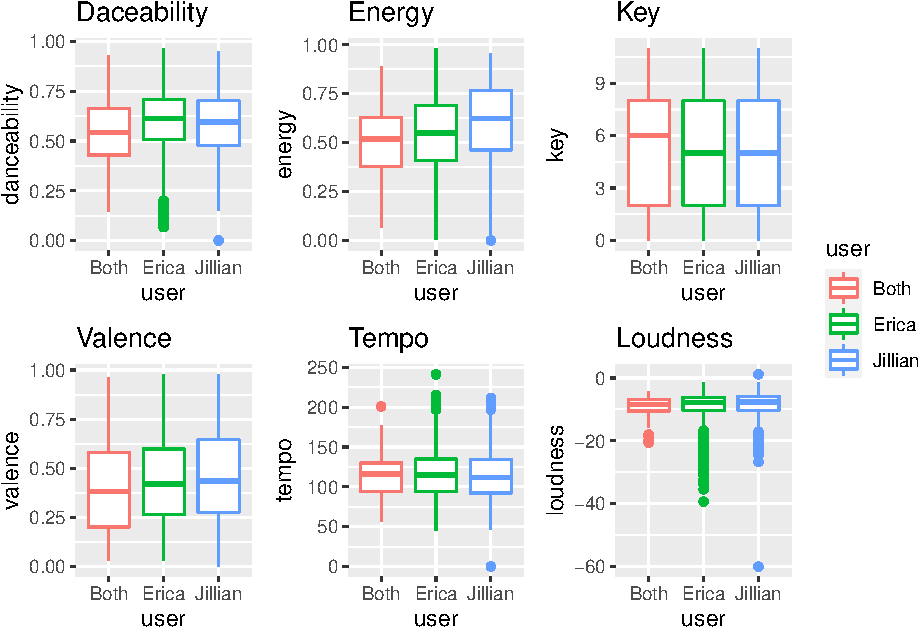
\includegraphics{lab5_files/figure-latex/unnamed-chunk-4-1.pdf} Based on
how similar these variables are across Jillian and me, it could be very
tough for the models to correctly classify tracks - but we'll see!

\hypertarget{modeling}{%
\subsubsection{\texorpdfstring{\textbf{Modeling}}{Modeling}}\label{modeling}}

\#Now with an added random forest component and some clarification your
task.

Create competing models that predict whether a track belongs to:

\textbf{Option 1. you or your partner's collection}

Option 2. genre 1 or genre 2

Create three final candidate models:

\begin{enumerate}
\def\labelenumi{\arabic{enumi}.}
\tightlist
\item
  k-nearest neighbor
\item
  decision tree
\item
  bagged tree

  \begin{itemize}
  \tightlist
  \item
    bag\_tree()
  \item
    Use the ``times ='' argument when setting the engine during model
    specification to specify the number of trees. The rule of thumb is
    that 50-500 trees is usually sufficient. The bottom of that range
    should be sufficient here.\\
  \end{itemize}
\item
  random forest

  \begin{itemize}
  \tightlist
  \item
    rand\_forest()
  \item
    m\_try() is the new hyperparameter of interest for this type of
    model. Make sure to include it in your tuning process
  \end{itemize}
\end{enumerate}

Go through the modeling process for each model:

Preprocessing. You can use the same recipe for all the models you
create.

Resampling. Make sure to use appropriate resampling to select the best
version created by each algorithm.

Tuning. Find the best values for each hyperparameter (within a
reasonable range).

Compare the performance of the four final models you have created.

Use appropriate performance evaluation metric(s) for this classification
task. A table would be a good way to display your comparison. Use at
least one visualization illustrating your model results

\hypertarget{pre-processing}{%
\subsection{Pre-Processing}\label{pre-processing}}

Splitting the data and encoding - this pre-processed data will be used
in each of the four models below.

\begin{Shaded}
\begin{Highlighting}[]
\CommentTok{\#remove unique identifiers from dataset (track id and song name)}
\NormalTok{tracks\_df }\OtherTok{\textless{}{-}}\NormalTok{ eb\_ja\_tracks }\SpecialCharTok{|\textgreater{}} 
  \FunctionTok{select}\NormalTok{(}\SpecialCharTok{{-}}\FunctionTok{c}\NormalTok{(id, track.name)) }\SpecialCharTok{|\textgreater{}} 
  \FunctionTok{mutate}\NormalTok{(}\AttributeTok{user =} \FunctionTok{as.factor}\NormalTok{(user)) }\CommentTok{\#make outcome variable a factor}

\CommentTok{\#split the data FIRST}
\FunctionTok{set.seed}\NormalTok{(}\DecValTok{123}\NormalTok{) }\CommentTok{\#set seed}

\NormalTok{tracks\_split }\OtherTok{\textless{}{-}} \FunctionTok{initial\_split}\NormalTok{(tracks\_df) }\CommentTok{\#split}
\NormalTok{tracks\_train }\OtherTok{\textless{}{-}} \FunctionTok{training}\NormalTok{(tracks\_split) }\CommentTok{\#training dataset}
\NormalTok{tracks\_test }\OtherTok{\textless{}{-}} \FunctionTok{testing}\NormalTok{(tracks\_split) }\CommentTok{\#testing dataset}

\CommentTok{\#Preprocess the data {-} encoding with the recipe}
\NormalTok{tracks\_recipe }\OtherTok{\textless{}{-}} \FunctionTok{recipe}\NormalTok{(user }\SpecialCharTok{\textasciitilde{}}\NormalTok{., }\AttributeTok{data =}\NormalTok{ tracks\_train) }\SpecialCharTok{|\textgreater{}} 
  \FunctionTok{step\_dummy}\NormalTok{(}\FunctionTok{all\_nominal}\NormalTok{(), }\SpecialCharTok{{-}}\FunctionTok{all\_outcomes}\NormalTok{(), }\AttributeTok{one\_hot =} \ConstantTok{TRUE}\NormalTok{) }\SpecialCharTok{|\textgreater{}} \CommentTok{\#one hot encoding of nominal variables ({-} user)}
  \FunctionTok{step\_normalize}\NormalTok{(}\FunctionTok{all\_numeric}\NormalTok{(), }\SpecialCharTok{{-}}\FunctionTok{all\_outcomes}\NormalTok{()) }\SpecialCharTok{|\textgreater{}} \CommentTok{\#normalize scale of numeric variables }
  \FunctionTok{prep}\NormalTok{()}
\end{Highlighting}
\end{Shaded}

Create re-sampling folds

\begin{Shaded}
\begin{Highlighting}[]
\CommentTok{\#resample}
\DocumentationTok{\#\# This resampling can be used for all of the models below!}
\FunctionTok{set.seed}\NormalTok{(}\DecValTok{123}\NormalTok{)}
\NormalTok{cv\_folds }\OtherTok{\textless{}{-}}\NormalTok{tracks\_train }\SpecialCharTok{|\textgreater{}} 
  \FunctionTok{vfold\_cv}\NormalTok{() }\CommentTok{\#10 folds is default}
\end{Highlighting}
\end{Shaded}

\hypertarget{knn-model}{%
\subsection{KNN Model}\label{knn-model}}

\begin{Shaded}
\begin{Highlighting}[]
\CommentTok{\#specify model}
\NormalTok{knn\_spec }\OtherTok{\textless{}{-}} \FunctionTok{nearest\_neighbor}\NormalTok{() }\SpecialCharTok{|\textgreater{}} \CommentTok{\#use defaults for first specification}
  \FunctionTok{set\_engine}\NormalTok{(}\StringTok{"kknn"}\NormalTok{) }\SpecialCharTok{|\textgreater{}} 
  \FunctionTok{set\_mode}\NormalTok{(}\StringTok{"classification"}\NormalTok{) }

\CommentTok{\#create a workflow}
\NormalTok{knn\_workflow }\OtherTok{\textless{}{-}} \FunctionTok{workflow}\NormalTok{() }\SpecialCharTok{|\textgreater{}} 
  \FunctionTok{add\_model}\NormalTok{(knn\_spec) }\SpecialCharTok{|\textgreater{}} 
  \FunctionTok{add\_recipe}\NormalTok{(tracks\_recipe)}
\end{Highlighting}
\end{Shaded}

\begin{Shaded}
\begin{Highlighting}[]
\CommentTok{\#fit resamples to the workflow}
\NormalTok{knn\_res }\OtherTok{\textless{}{-}} 
\NormalTok{  knn\_workflow }\SpecialCharTok{|\textgreater{}} 
  \FunctionTok{fit\_resamples}\NormalTok{( }\CommentTok{\#tuning function}
    \AttributeTok{resamples =}\NormalTok{ cv\_folds,}
    \AttributeTok{control =} \FunctionTok{control\_resamples}\NormalTok{(}\AttributeTok{save\_pred =} \ConstantTok{TRUE}\NormalTok{) }\CommentTok{\#save prediction}
\NormalTok{    )}

\CommentTok{\# Now define our KNN model with tuning}
\NormalTok{knn\_spec\_tune }\OtherTok{\textless{}{-}} 
  \FunctionTok{nearest\_neighbor}\NormalTok{(}\AttributeTok{neighbors =} \FunctionTok{tune}\NormalTok{()) }\SpecialCharTok{|\textgreater{}}  \CommentTok{\#now specify how many neighbors {-} use tune to look for best}
  \FunctionTok{set\_mode}\NormalTok{(}\StringTok{"classification"}\NormalTok{) }\SpecialCharTok{|\textgreater{}} 
  \FunctionTok{set\_engine}\NormalTok{(}\StringTok{"kknn"}\NormalTok{)}

\CommentTok{\# Define a new workflow}
\NormalTok{wf\_knn\_tune }\OtherTok{\textless{}{-}} \FunctionTok{workflow}\NormalTok{() }\SpecialCharTok{|\textgreater{}} 
  \FunctionTok{add\_model}\NormalTok{(knn\_spec\_tune) }\SpecialCharTok{|\textgreater{}} 
  \FunctionTok{add\_recipe}\NormalTok{(tracks\_recipe) }

\CommentTok{\# Fit the workflow on our predefined folds and hyperparameters}
\NormalTok{fit\_knn\_cv }\OtherTok{\textless{}{-}}\NormalTok{ wf\_knn\_tune }\SpecialCharTok{|\textgreater{}} 
  \FunctionTok{tune\_grid}\NormalTok{( }
\NormalTok{    cv\_folds,}
    \AttributeTok{grid =} \FunctionTok{data.frame}\NormalTok{(}\AttributeTok{neighbors =} \FunctionTok{c}\NormalTok{(}\DecValTok{1}\NormalTok{, }\DecValTok{5}\NormalTok{, }\FunctionTok{seq}\NormalTok{(}\DecValTok{10}\NormalTok{,}\DecValTok{100}\NormalTok{,}\DecValTok{10}\NormalTok{)))) }
\end{Highlighting}
\end{Shaded}

\begin{Shaded}
\begin{Highlighting}[]
\CommentTok{\# The final workflow for our KNN model}
\NormalTok{final\_knn\_wf }\OtherTok{\textless{}{-}} 
\NormalTok{  knn\_workflow }\SpecialCharTok{|\textgreater{}} 
  \FunctionTok{finalize\_workflow}\NormalTok{(}\FunctionTok{select\_best}\NormalTok{(fit\_knn\_cv))}
\end{Highlighting}
\end{Shaded}

\begin{verbatim}
## Warning: No value of `metric` was given; metric 'roc_auc' will be used.
\end{verbatim}

\begin{Shaded}
\begin{Highlighting}[]
\CommentTok{\# \# Fitting our final workflow}
\NormalTok{final\_knn\_fit }\OtherTok{\textless{}{-}}\NormalTok{ final\_knn\_wf }\SpecialCharTok{|\textgreater{}} 
  \FunctionTok{last\_fit}\NormalTok{(tracks\_split) }

\CommentTok{\# Collect metrics}
\NormalTok{knn\_metrics }\OtherTok{\textless{}{-}}\NormalTok{ final\_knn\_fit }\SpecialCharTok{|\textgreater{}} \FunctionTok{collect\_metrics}\NormalTok{()}
\end{Highlighting}
\end{Shaded}

\hypertarget{decision-tree}{%
\subsection{Decision Tree}\label{decision-tree}}

\begin{Shaded}
\begin{Highlighting}[]
\CommentTok{\#create a model with with tuning specifications}
\NormalTok{tree\_spec\_tune }\OtherTok{\textless{}{-}} \FunctionTok{decision\_tree}\NormalTok{(}
  \AttributeTok{cost\_complexity =} \FunctionTok{tune}\NormalTok{(),}
  \AttributeTok{tree\_depth =} \FunctionTok{tune}\NormalTok{(),}
  \AttributeTok{min\_n =} \FunctionTok{tune}\NormalTok{()}
\NormalTok{) }\SpecialCharTok{|\textgreater{}} 
  \FunctionTok{set\_engine}\NormalTok{(}\StringTok{"rpart"}\NormalTok{) }\SpecialCharTok{|\textgreater{}} 
  \FunctionTok{set\_mode}\NormalTok{(}\StringTok{"classification"}\NormalTok{)}

\CommentTok{\#test out some hyperparameters in a search grid}
\NormalTok{tree\_grid }\OtherTok{\textless{}{-}} \FunctionTok{grid\_regular}\NormalTok{(}\FunctionTok{cost\_complexity}\NormalTok{(), }\FunctionTok{tree\_depth}\NormalTok{(),}
                          \FunctionTok{min\_n}\NormalTok{(),}
                          \AttributeTok{levels =} \DecValTok{3}\NormalTok{) }\CommentTok{\#27 total outcomes to try}

\NormalTok{tree\_grid}
\end{Highlighting}
\end{Shaded}

\begin{verbatim}
## # A tibble: 27 x 3
##    cost_complexity tree_depth min_n
##              <dbl>      <int> <int>
##  1    0.0000000001          1     2
##  2    0.00000316            1     2
##  3    0.1                   1     2
##  4    0.0000000001          8     2
##  5    0.00000316            8     2
##  6    0.1                   8     2
##  7    0.0000000001         15     2
##  8    0.00000316           15     2
##  9    0.1                  15     2
## 10    0.0000000001          1    21
## # ... with 17 more rows
## # i Use `print(n = ...)` to see more rows
\end{verbatim}

\begin{Shaded}
\begin{Highlighting}[]
\CommentTok{\#add tree specifications to a workflow}
\NormalTok{wf\_tree\_tune }\OtherTok{\textless{}{-}} \FunctionTok{workflow}\NormalTok{() }\SpecialCharTok{|\textgreater{}} 
  \FunctionTok{add\_recipe}\NormalTok{(tracks\_recipe) }\SpecialCharTok{|\textgreater{}} 
  \FunctionTok{add\_model}\NormalTok{(tree\_spec\_tune)}


\NormalTok{doParallel}\SpecialCharTok{::}\FunctionTok{registerDoParallel}\NormalTok{() }\CommentTok{\#build trees in parallel}

\NormalTok{tree\_rs }\OtherTok{\textless{}{-}} \FunctionTok{tune\_grid}\NormalTok{(}
\NormalTok{  tree\_spec\_tune,}
\NormalTok{  user}\SpecialCharTok{\textasciitilde{}}\NormalTok{.,}
  \AttributeTok{resamples =}\NormalTok{ cv\_folds,}
  \AttributeTok{grid =}\NormalTok{ tree\_grid,}
  \AttributeTok{metrics =} \FunctionTok{metric\_set}\NormalTok{(accuracy)}
\NormalTok{)}

\NormalTok{tree\_rs}
\end{Highlighting}
\end{Shaded}

\begin{verbatim}
## # Tuning results
## # 10-fold cross-validation 
## # A tibble: 10 x 4
##    splits             id     .metrics          .notes          
##    <list>             <chr>  <list>            <list>          
##  1 <split [2542/283]> Fold01 <tibble [27 x 7]> <tibble [0 x 3]>
##  2 <split [2542/283]> Fold02 <tibble [27 x 7]> <tibble [0 x 3]>
##  3 <split [2542/283]> Fold03 <tibble [27 x 7]> <tibble [0 x 3]>
##  4 <split [2542/283]> Fold04 <tibble [27 x 7]> <tibble [0 x 3]>
##  5 <split [2542/283]> Fold05 <tibble [27 x 7]> <tibble [0 x 3]>
##  6 <split [2543/282]> Fold06 <tibble [27 x 7]> <tibble [0 x 3]>
##  7 <split [2543/282]> Fold07 <tibble [27 x 7]> <tibble [0 x 3]>
##  8 <split [2543/282]> Fold08 <tibble [27 x 7]> <tibble [0 x 3]>
##  9 <split [2543/282]> Fold09 <tibble [27 x 7]> <tibble [0 x 3]>
## 10 <split [2543/282]> Fold10 <tibble [27 x 7]> <tibble [0 x 3]>
\end{verbatim}

\begin{Shaded}
\begin{Highlighting}[]
\CommentTok{\#check out resampled models}

\FunctionTok{autoplot}\NormalTok{(tree\_rs) }\SpecialCharTok{+}
  \FunctionTok{theme\_minimal}\NormalTok{()}
\end{Highlighting}
\end{Shaded}

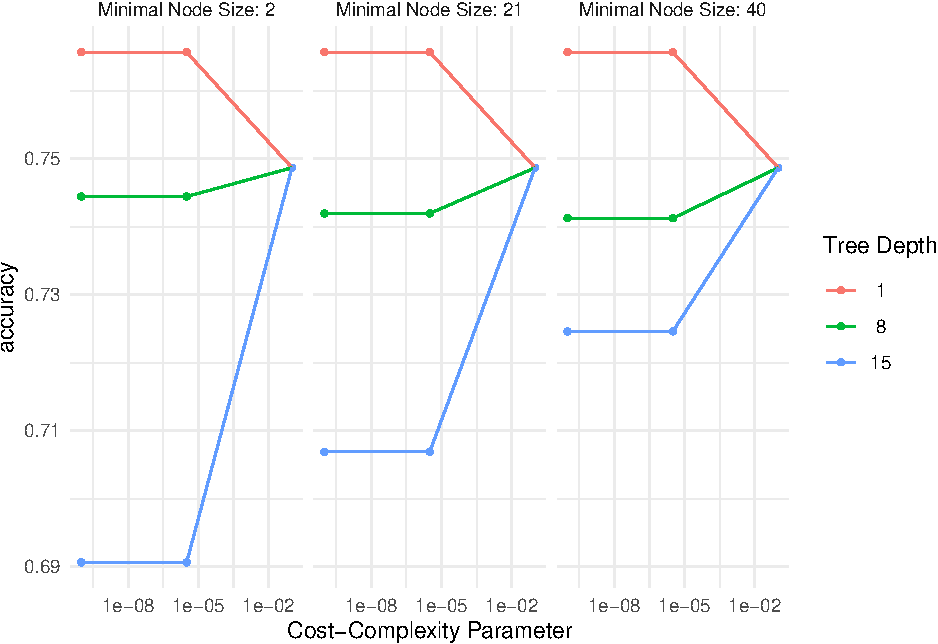
\includegraphics{lab5_files/figure-latex/unnamed-chunk-5-1.pdf}

\begin{Shaded}
\begin{Highlighting}[]
\FunctionTok{show\_best}\NormalTok{(tree\_rs) }\CommentTok{\#show me the best tree! }
\end{Highlighting}
\end{Shaded}

\begin{verbatim}
## # A tibble: 5 x 9
##   cost_complexity tree_depth min_n .metric  .estim~1  mean     n std_err .config
##             <dbl>      <int> <int> <chr>    <chr>    <dbl> <int>   <dbl> <chr>  
## 1    0.0000000001          1     2 accuracy multicl~ 0.766    10 0.00676 Prepro~
## 2    0.00000316            1     2 accuracy multicl~ 0.766    10 0.00676 Prepro~
## 3    0.0000000001          1    21 accuracy multicl~ 0.766    10 0.00676 Prepro~
## 4    0.00000316            1    21 accuracy multicl~ 0.766    10 0.00676 Prepro~
## 5    0.0000000001          1    40 accuracy multicl~ 0.766    10 0.00676 Prepro~
## # ... with abbreviated variable name 1: .estimator
\end{verbatim}

\begin{Shaded}
\begin{Highlighting}[]
\FunctionTok{select\_best}\NormalTok{(tree\_rs) }\CommentTok{\#pick the best tree}
\end{Highlighting}
\end{Shaded}

\begin{verbatim}
## # A tibble: 1 x 4
##   cost_complexity tree_depth min_n .config              
##             <dbl>      <int> <int> <chr>                
## 1    0.0000000001          1     2 Preprocessor1_Model01
\end{verbatim}

As shown in the plot above and the output from the \texttt{select\_best}
tree function, my best model has a tree depth of just one. I suspect
this is because the tracks in the two user groups are so similar so the
greater depth is adding variance and making the model worse.

\begin{Shaded}
\begin{Highlighting}[]
\NormalTok{final\_tree }\OtherTok{\textless{}{-}} \FunctionTok{finalize\_model}\NormalTok{(tree\_spec\_tune, }\FunctionTok{select\_best}\NormalTok{(tree\_rs)) }\CommentTok{\#finalize model}

\CommentTok{\#show the predictions from this final model}
\NormalTok{final\_tree\_fit }\OtherTok{\textless{}{-}} \FunctionTok{last\_fit}\NormalTok{(final\_tree, }
\NormalTok{                           user}\SpecialCharTok{\textasciitilde{}}\NormalTok{.,}
\NormalTok{                           tracks\_split)}

\NormalTok{final\_tree\_fit}\SpecialCharTok{$}\NormalTok{.predictions}
\end{Highlighting}
\end{Shaded}

\begin{verbatim}
## [[1]]
## # A tibble: 942 x 7
##    .pred_Both .pred_Erica .pred_Jillian  .row .pred_class user  .config         
##         <dbl>       <dbl>         <dbl> <int> <fct>       <fct> <chr>           
##  1     0.0336       0.763         0.203     3 Erica       Erica Preprocessor1_M~
##  2     0.0336       0.763         0.203     6 Erica       Erica Preprocessor1_M~
##  3     0.0336       0.763         0.203    14 Erica       Erica Preprocessor1_M~
##  4     0.0336       0.763         0.203    22 Erica       Erica Preprocessor1_M~
##  5     0.0336       0.763         0.203    43 Erica       Erica Preprocessor1_M~
##  6     0.0336       0.763         0.203    47 Erica       Erica Preprocessor1_M~
##  7     0.0336       0.763         0.203    50 Erica       Erica Preprocessor1_M~
##  8     0.0336       0.763         0.203    53 Erica       Erica Preprocessor1_M~
##  9     0.0336       0.763         0.203    55 Erica       Erica Preprocessor1_M~
## 10     0.0336       0.763         0.203    57 Erica       Erica Preprocessor1_M~
## # ... with 932 more rows
## # i Use `print(n = ...)` to see more rows
\end{verbatim}

\begin{Shaded}
\begin{Highlighting}[]
\NormalTok{tree\_metrics }\OtherTok{\textless{}{-}} \FunctionTok{collect\_metrics}\NormalTok{(final\_tree\_fit)}
\end{Highlighting}
\end{Shaded}

\hypertarget{bagged-tree}{%
\subsection{Bagged Tree}\label{bagged-tree}}

\begin{Shaded}
\begin{Highlighting}[]
\CommentTok{\#specify model without tuning parameters (using defaults)}
\NormalTok{bag\_spec }\OtherTok{\textless{}{-}} \FunctionTok{bag\_tree}\NormalTok{() }\SpecialCharTok{|\textgreater{}} 
  \FunctionTok{set\_engine}\NormalTok{(}\StringTok{"rpart"}\NormalTok{, }\AttributeTok{times =} \DecValTok{50}\NormalTok{) }\SpecialCharTok{|\textgreater{}} 
  \FunctionTok{set\_mode}\NormalTok{(}\StringTok{"classification"}\NormalTok{)}

\CommentTok{\#with tuning = takes 5ever}
\NormalTok{bag\_spec\_tune }\OtherTok{\textless{}{-}} \FunctionTok{bag\_tree}\NormalTok{(}
  \AttributeTok{cost\_complexity =} \FunctionTok{tune}\NormalTok{(),}
  \AttributeTok{tree\_depth =} \FunctionTok{tune}\NormalTok{(),}
  \AttributeTok{min\_n =} \FunctionTok{tune}\NormalTok{()}
\NormalTok{) }\SpecialCharTok{|\textgreater{}} 
  \FunctionTok{set\_engine}\NormalTok{(}\StringTok{"rpart"}\NormalTok{, }\AttributeTok{times =} \DecValTok{50}\NormalTok{) }\SpecialCharTok{|\textgreater{}} 
  \FunctionTok{set\_mode}\NormalTok{(}\StringTok{"classification"}\NormalTok{)}

\CommentTok{\#create hyperparameter search grid}
\NormalTok{bagrid }\OtherTok{\textless{}{-}} \FunctionTok{grid\_regular}\NormalTok{(}
  \FunctionTok{cost\_complexity}\NormalTok{(),}
  \FunctionTok{tree\_depth}\NormalTok{(),}
  \FunctionTok{min\_n}\NormalTok{(),}
  \AttributeTok{levels =} \DecValTok{5}
\NormalTok{)}

\CommentTok{\#wrap up into a workflow}
\NormalTok{wf\_bag\_tune }\OtherTok{\textless{}{-}} \FunctionTok{workflow}\NormalTok{() }\SpecialCharTok{|\textgreater{}} 
  \FunctionTok{add\_recipe}\NormalTok{(tracks\_recipe) }\SpecialCharTok{|\textgreater{}} 
  \FunctionTok{add\_model}\NormalTok{(bag\_spec\_tune)}
\end{Highlighting}
\end{Shaded}

\begin{Shaded}
\begin{Highlighting}[]
\CommentTok{\# \#trying to make this faster by using more cores than default:}
\CommentTok{\# ncores \textless{}{-} detectCores() {-} 1 \#use one less than the number of cores on my machine}
\CommentTok{\# registerDoParallel(cores = ncores) \#register this number of cores}
\CommentTok{\# cl \textless{}{-} makeCluster(ncores, type = "FORK") \#make cluster with fork}
\CommentTok{\# registerDoParallel(cl)}

\CommentTok{\#using taylor to knit instead so hopefully basic function will work:}
\NormalTok{doParallel}\SpecialCharTok{::}\FunctionTok{registerDoParallel}\NormalTok{()}

\CommentTok{\#fit workflow to resamples}
\NormalTok{bag\_rs }\OtherTok{\textless{}{-}} \FunctionTok{tune\_grid}\NormalTok{(}
\NormalTok{  bag\_spec\_tune,}
\NormalTok{  user }\SpecialCharTok{\textasciitilde{}}\NormalTok{.,}
  \AttributeTok{resamples =}\NormalTok{ cv\_folds,}
  \AttributeTok{grid =}\NormalTok{ bagrid,}
  \AttributeTok{metrics =} \FunctionTok{metric\_set}\NormalTok{(accuracy)}
\NormalTok{)}
\CommentTok{\# stopCluster(cl) \#manually stop clusters}
\CommentTok{\# stopImplicitCluster() \#running into problems {-} hopefully this stops it better??}
\end{Highlighting}
\end{Shaded}

\begin{Shaded}
\begin{Highlighting}[]
\NormalTok{final\_bag }\OtherTok{\textless{}{-}} \FunctionTok{finalize\_model}\NormalTok{(bag\_spec\_tune, }\FunctionTok{select\_best}\NormalTok{(bag\_rs)) }\CommentTok{\#finalize model}

\CommentTok{\#show the predictions from this final model}
\NormalTok{final\_bag\_fit }\OtherTok{\textless{}{-}} \FunctionTok{last\_fit}\NormalTok{(final\_bag, }
\NormalTok{                           user}\SpecialCharTok{\textasciitilde{}}\NormalTok{.,}
\NormalTok{                           tracks\_split)}

\NormalTok{final\_bag\_fit}\SpecialCharTok{$}\NormalTok{.predictions }\CommentTok{\#look at some predictions if you want if you care}
\end{Highlighting}
\end{Shaded}

\begin{verbatim}
## [[1]]
## # A tibble: 942 x 7
##    .pred_Both .pred_Erica .pred_Jillian  .row .pred_class user  .config         
##         <dbl>       <dbl>         <dbl> <int> <fct>       <fct> <chr>           
##  1    0.0412        0.485        0.473      3 Erica       Erica Preprocessor1_M~
##  2    0.00901       0.765        0.226      6 Erica       Erica Preprocessor1_M~
##  3    0.0186        0.868        0.114     14 Erica       Erica Preprocessor1_M~
##  4    0.0641        0.674        0.262     22 Erica       Erica Preprocessor1_M~
##  5    0.0488        0.864        0.0869    43 Erica       Erica Preprocessor1_M~
##  6    0.0103        0.748        0.241     47 Erica       Erica Preprocessor1_M~
##  7    0.0369        0.826        0.138     50 Erica       Erica Preprocessor1_M~
##  8    0.0130        0.930        0.0570    53 Erica       Erica Preprocessor1_M~
##  9    0.00530       0.891        0.104     55 Erica       Erica Preprocessor1_M~
## 10    0.0351        0.858        0.107     57 Erica       Erica Preprocessor1_M~
## # ... with 932 more rows
## # i Use `print(n = ...)` to see more rows
\end{verbatim}

\begin{Shaded}
\begin{Highlighting}[]
\NormalTok{bag\_metrics }\OtherTok{\textless{}{-}} \FunctionTok{collect\_metrics}\NormalTok{(final\_bag\_fit)}
\end{Highlighting}
\end{Shaded}

\hypertarget{random-forest}{%
\subsection{Random Forest}\label{random-forest}}

\begin{Shaded}
\begin{Highlighting}[]
\CommentTok{\#specify model}

\NormalTok{rand\_spec\_tune }\OtherTok{\textless{}{-}} \FunctionTok{rand\_forest}\NormalTok{(}
  \AttributeTok{mtry =} \FunctionTok{tune}\NormalTok{(), }\CommentTok{\#using sqrt(p) = 4 for mtry}
  \AttributeTok{trees =} \DecValTok{1000}\NormalTok{, }\CommentTok{\#using default number}
  \AttributeTok{min\_n =} \FunctionTok{tune}\NormalTok{() }
\NormalTok{) }\SpecialCharTok{|\textgreater{}} 
  \FunctionTok{set\_engine}\NormalTok{(}\StringTok{"ranger"}\NormalTok{) }\SpecialCharTok{|\textgreater{}} 
  \FunctionTok{set\_mode}\NormalTok{(}\StringTok{"classification"}\NormalTok{)}

\CommentTok{\# put into a workflow}
\NormalTok{wf\_rand\_tune }\OtherTok{\textless{}{-}} \FunctionTok{workflow}\NormalTok{() }\SpecialCharTok{|\textgreater{}} 
  \FunctionTok{add\_recipe}\NormalTok{(tracks\_recipe) }\SpecialCharTok{|\textgreater{}} 
  \FunctionTok{add\_model}\NormalTok{(rand\_spec\_tune)}

\CommentTok{\#train hyperparameters}

\CommentTok{\#set up paralelle again}
\NormalTok{doParallel}\SpecialCharTok{::}\FunctionTok{registerDoParallel}\NormalTok{()}
\FunctionTok{set.seed}\NormalTok{(}\DecValTok{321}\NormalTok{)}
\NormalTok{rand\_tune\_res }\OtherTok{\textless{}{-}} \FunctionTok{tune\_grid}\NormalTok{(}
\NormalTok{  wf\_rand\_tune,}
  \AttributeTok{resamples =}\NormalTok{ cv\_folds,}
  \AttributeTok{grid =} \DecValTok{20} \CommentTok{\#testing 20 points to tune}
\NormalTok{)}
\end{Highlighting}
\end{Shaded}

\begin{verbatim}
## i Creating pre-processing data to finalize unknown parameter: mtry
\end{verbatim}

\begin{Shaded}
\begin{Highlighting}[]
\CommentTok{\#select the best parameters}
\NormalTok{rand\_tune\_best }\OtherTok{\textless{}{-}}\NormalTok{ rand\_tune\_res }\SpecialCharTok{|\textgreater{}} 
  \FunctionTok{select\_best}\NormalTok{(}\StringTok{"accuracy"}\NormalTok{)}
\end{Highlighting}
\end{Shaded}

\begin{Shaded}
\begin{Highlighting}[]
\NormalTok{final\_rand }\OtherTok{\textless{}{-}} \FunctionTok{finalize\_model}\NormalTok{(rand\_spec\_tune, }\FunctionTok{select\_best}\NormalTok{(rand\_tune\_res)) }\CommentTok{\#finalize model}
\end{Highlighting}
\end{Shaded}

\begin{verbatim}
## Warning: No value of `metric` was given; metric 'roc_auc' will be used.
\end{verbatim}

\begin{Shaded}
\begin{Highlighting}[]
\CommentTok{\#show the predictions from this final model}
\NormalTok{final\_rand\_fit }\OtherTok{\textless{}{-}} \FunctionTok{last\_fit}\NormalTok{(final\_rand, }
\NormalTok{                           user}\SpecialCharTok{\textasciitilde{}}\NormalTok{.,}
\NormalTok{                           tracks\_split)}

\NormalTok{final\_rand\_fit}\SpecialCharTok{$}\NormalTok{.predictions }\CommentTok{\#look at some predictions if you want if you care}
\end{Highlighting}
\end{Shaded}

\begin{verbatim}
## [[1]]
## # A tibble: 942 x 7
##    .pred_Both .pred_Erica .pred_Jillian  .row .pred_class user  .config         
##         <dbl>       <dbl>         <dbl> <int> <fct>       <fct> <chr>           
##  1     0.034        0.611        0.355      3 Erica       Erica Preprocessor1_M~
##  2     0.025        0.74         0.235      6 Erica       Erica Preprocessor1_M~
##  3     0.0402       0.857        0.103     14 Erica       Erica Preprocessor1_M~
##  4     0.0375       0.679        0.283     22 Erica       Erica Preprocessor1_M~
##  5     0.061        0.839        0.0997    43 Erica       Erica Preprocessor1_M~
##  6     0.0555       0.732        0.212     47 Erica       Erica Preprocessor1_M~
##  7     0.0455       0.793        0.161     50 Erica       Erica Preprocessor1_M~
##  8     0.0177       0.917        0.0652    53 Erica       Erica Preprocessor1_M~
##  9     0.0263       0.892        0.0817    55 Erica       Erica Preprocessor1_M~
## 10     0.0497       0.738        0.213     57 Erica       Erica Preprocessor1_M~
## # ... with 932 more rows
## # i Use `print(n = ...)` to see more rows
\end{verbatim}

\begin{Shaded}
\begin{Highlighting}[]
\NormalTok{rand\_metrics }\OtherTok{\textless{}{-}} \FunctionTok{collect\_metrics}\NormalTok{(final\_rand\_fit)}
\end{Highlighting}
\end{Shaded}

\hypertarget{comparing-the-models}{%
\section{Comparing the models}\label{comparing-the-models}}

Compare the performance of the four final models you have created.

Use appropriate performance evaluation metric(s) for this classification
task. A table would be a good way to display your comparison. Use at
least one visualization illustrating your model results

\begin{Shaded}
\begin{Highlighting}[]
\CommentTok{\#compare metrics}
\NormalTok{knn\_metrics}
\end{Highlighting}
\end{Shaded}

\begin{verbatim}
## # A tibble: 2 x 4
##   .metric  .estimator .estimate .config             
##   <chr>    <chr>          <dbl> <chr>               
## 1 accuracy multiclass     0.726 Preprocessor1_Model1
## 2 roc_auc  hand_till      0.610 Preprocessor1_Model1
\end{verbatim}

\begin{Shaded}
\begin{Highlighting}[]
\NormalTok{tree\_metrics}
\end{Highlighting}
\end{Shaded}

\begin{verbatim}
## # A tibble: 2 x 4
##   .metric  .estimator .estimate .config             
##   <chr>    <chr>          <dbl> <chr>               
## 1 accuracy multiclass     0.791 Preprocessor1_Model1
## 2 roc_auc  hand_till      0.541 Preprocessor1_Model1
\end{verbatim}

\begin{Shaded}
\begin{Highlighting}[]
\NormalTok{bag\_metrics}
\end{Highlighting}
\end{Shaded}

\begin{verbatim}
## # A tibble: 2 x 4
##   .metric  .estimator .estimate .config             
##   <chr>    <chr>          <dbl> <chr>               
## 1 accuracy multiclass     0.800 Preprocessor1_Model1
## 2 roc_auc  hand_till      0.624 Preprocessor1_Model1
\end{verbatim}

\begin{Shaded}
\begin{Highlighting}[]
\NormalTok{rand\_metrics}
\end{Highlighting}
\end{Shaded}

\begin{verbatim}
## # A tibble: 2 x 4
##   .metric  .estimator .estimate .config             
##   <chr>    <chr>          <dbl> <chr>               
## 1 accuracy multiclass     0.801 Preprocessor1_Model1
## 2 roc_auc  hand_till      0.647 Preprocessor1_Model1
\end{verbatim}

\begin{Shaded}
\begin{Highlighting}[]
\CommentTok{\#create table comparing accuracy metrics}
\NormalTok{accuracy\_tibble }\OtherTok{\textless{}{-}} \FunctionTok{tibble}\NormalTok{(}
  \AttributeTok{model =} \FunctionTok{c}\NormalTok{(}\StringTok{"knn"}\NormalTok{, }\StringTok{"decision\_tree"}\NormalTok{, }\StringTok{"bagged\_tree"}\NormalTok{, }\StringTok{"random\_forest"}\NormalTok{),}
  \AttributeTok{accuracy =} \FunctionTok{c}\NormalTok{(}\FunctionTok{round}\NormalTok{(knn\_metrics[}\DecValTok{1}\NormalTok{, }\DecValTok{3}\NormalTok{], }\DecValTok{3}\NormalTok{), }\FunctionTok{round}\NormalTok{(tree\_metrics[}\DecValTok{1}\NormalTok{, }\DecValTok{3}\NormalTok{], }\DecValTok{3}\NormalTok{), }\FunctionTok{round}\NormalTok{(bag\_metrics[}\DecValTok{1}\NormalTok{, }\DecValTok{3}\NormalTok{], }\DecValTok{3}\NormalTok{), }\FunctionTok{round}\NormalTok{(rand\_metrics[}\DecValTok{1}\NormalTok{, }\DecValTok{3}\NormalTok{], }\DecValTok{3}\NormalTok{)),}
  \AttributeTok{area\_under\_curve =} \FunctionTok{c}\NormalTok{(}\FunctionTok{round}\NormalTok{(knn\_metrics[}\DecValTok{2}\NormalTok{, }\DecValTok{3}\NormalTok{], }\DecValTok{3}\NormalTok{), }\FunctionTok{round}\NormalTok{(tree\_metrics[}\DecValTok{2}\NormalTok{, }\DecValTok{3}\NormalTok{], }\DecValTok{3}\NormalTok{), }\FunctionTok{round}\NormalTok{(bag\_metrics[}\DecValTok{2}\NormalTok{, }\DecValTok{3}\NormalTok{], }\DecValTok{3}\NormalTok{), }\FunctionTok{round}\NormalTok{(rand\_metrics[}\DecValTok{2}\NormalTok{, }\DecValTok{3}\NormalTok{], }\DecValTok{3}\NormalTok{))}
\NormalTok{)}

\FunctionTok{gt}\NormalTok{(accuracy\_tibble)}
\end{Highlighting}
\end{Shaded}

\begin{longtable}{lcc}
\toprule
model & accuracy & area\_under\_curve \\ 
\midrule
knn & 0.726 & 0.61 \\ 
decision\_tree & 0.791 & 0.541 \\ 
bagged\_tree & 0.8 & 0.624 \\ 
random\_forest & 0.801 & 0.647 \\ 
\bottomrule
\end{longtable}

\begin{Shaded}
\begin{Highlighting}[]
\CommentTok{\#visualize accuracy}
\FunctionTok{ggplot}\NormalTok{(}\AttributeTok{data =}\NormalTok{ accuracy\_tibble,}
       \FunctionTok{aes}\NormalTok{(}\AttributeTok{x =}\NormalTok{ model,}
           \AttributeTok{y =}\NormalTok{ accuracy,}
           \AttributeTok{fill =}\NormalTok{ model)) }\SpecialCharTok{+}
  \FunctionTok{geom\_col}\NormalTok{() }\SpecialCharTok{+}
  \FunctionTok{labs}\NormalTok{(}
    \AttributeTok{title =} \StringTok{"comparing the accuracy of four machine learning models"}
\NormalTok{  )}
\end{Highlighting}
\end{Shaded}

\includegraphics{lab5_files/figure-latex/unnamed-chunk-8-1.pdf}

The greatest accuracy and the greatest area under the curve came from
the random forest model. It's not surprising that this preformed much
better than a single decision tree because a forest has lower bias than
a single tree. The Bagging preformed similarly, and probably could have
been tuned to preform even better than it did but the computation time
trade off wasn't worth it. I'm a little surprised that the KNN model
preformed worst, even worse than the single decision tree. I think this
is because in the case of which songs belong to which user, the
similarity of songs may not be the best predictor - especially becuase
Jillian and I both seem to have similar music preferences in terms of
the features used in this model.

\end{document}
